\newcommand{\plotGammasLambdas}[4]{
  % defines the pgfplots style "gammaslambdasdefault"
\pgfkeys{/pgfplots/gammaslambdasdefault/.style={
    width=1.0\linewidth,
    height=0.6\linewidth,
    every axis plot/.append style={line width = 1.5pt},
    mark size = 0.6,
    tick pos = left,
    ylabel near ticks,
    xlabel near ticks,
    xtick align = inside,
    ytick align = inside,
    legend cell align = left,
    legend columns = 1,
    legend pos = south east,
    legend style = {
      fill opacity = 0.7,
      text opacity = 1,
      font = \footnotesize,
    },
    xticklabel style = {font = \footnotesize},
    xlabel style = {font = \footnotesize},
    axis line style = {black},
    yticklabel style = {font = \footnotesize},
    ylabel style = {font = \footnotesize},
    title style = {font = \footnotesize},
    grid = major,
    grid style = {dashed}
  }
}
%%% Local Variables:
%%% mode: latex
%%% TeX-master: "../../thesis"
%%% End:

  \pgfkeys{/pgfplots/zmystyle/.style={
      gammaslambdasdefault,
    }}
  \input{../../fig/exp13_full_batch_monitoring/results/plots/gammas_lambdas/#1_#2_#3_#4}
}

\begin{figure}[p]
\centering
\textbf{\fmnist \twoctwod \sgd}\\[1mm]
\begin{minipage}{0.50\textwidth}
\centering
\plotGammasLambdas{fmnist}{2c2d}{sgd}{gammas}
% \includegraphics[scale=1.0]{fig/exp13_plots/gammas_lambdas/fmnist_2c2d_sgd_gammas.pdf}
\end{minipage}\hfill
\begin{minipage}{0.50\textwidth}
\centering
\plotGammasLambdas{fmnist}{2c2d}{sgd}{lambdas}
% \includegraphics[scale=1.0]{fig/exp13_plots/gammas_lambdas/fmnist_2c2d_sgd_lambdas.pdf}
\end{minipage}

\textbf{\fmnist \twoctwod \adam}\\[1mm]
\begin{minipage}{0.50\textwidth}
\centering
\plotGammasLambdas{fmnist}{2c2d}{adam}{gammas}
% \includegraphics[scale=1.0]{fig/exp13_plots/gammas_lambdas/fmnist_2c2d_adam_gammas.pdf}
\end{minipage}\hfill
\begin{minipage}{0.50\textwidth}
\centering
\plotGammasLambdas{fmnist}{2c2d}{adam}{lambdas}
% \includegraphics[scale=1.0]{fig/exp13_plots/gammas_lambdas/fmnist_2c2d_adam_lambdas.pdf}
\end{minipage}

\textbf{\cifarten \threecthreed \sgd}\\[1mm]
\begin{minipage}{0.50\textwidth}
\centering
\plotGammasLambdas{cifar10}{3c3d}{sgd}{gammas}
% \includegraphics[scale=1.0]{fig/exp13_plots/gammas_lambdas/cifar10_3c3d_sgd_gammas.pdf}
\end{minipage}\hfill
\begin{minipage}{0.50\textwidth}
\centering
\plotGammasLambdas{cifar10}{3c3d}{sgd}{lambdas}
% \includegraphics[scale=1.0]{fig/exp13_plots/gammas_lambdas/cifar10_3c3d_sgd_lambdas.pdf}
\end{minipage}

\textbf{\cifarten \threecthreed \adam}\\[1mm]
\begin{minipage}{0.50\textwidth}
\centering
\plotGammasLambdas{cifar10}{3c3d}{adam}{gammas}
% \includegraphics[scale=1.0]{fig/exp13_plots/gammas_lambdas/cifar10_3c3d_adam_gammas.pdf}
\end{minipage}\hfill
\begin{minipage}{0.50\textwidth}
\centering
\plotGammasLambdas{cifar10}{3c3d}{adam}{lambdas}
% \includegraphics[scale=1.0]{fig/exp13_plots/gammas_lambdas/cifar10_3c3d_adam_lambdas.pdf}
\end{minipage}

\vspace{-2mm}

\caption{\textbf{Directional SNRs (1):}
SNR along each of the mini-batch \ggn{}'s top-$C$ eigenvectors during training for all test problems.
At fixed epoch, the SNR for the most curved direction is shown in
{\protect\tikz{\protect\draw[white,fill={light_red},line width=0mm] (0,0) circle (.8ex);}}
and for the least curved direction in
{\protect\tikz{\protect\draw[white,fill={black}] (0,0) circle (.8ex);}}.
}

\label{fig:directional_derivatives_1}
\end{figure}



%=================================================================



\begin{figure}[p]
\centering
\textbf{\cifarten \resnetthirtytwo \sgd}\\[1mm]
\begin{minipage}{0.50\textwidth}
\centering
\plotGammasLambdas{cifar10}{resnet32}{sgd}{gammas}
% \includegraphics[scale=1.0]{fig/exp13_plots/gammas_lambdas/cifar10_resnet32_sgd_gammas.pdf}
\end{minipage}\hfill
\begin{minipage}{0.50\textwidth}
\centering
\plotGammasLambdas{cifar10}{resnet32}{sgd}{lambdas}
% \includegraphics[scale=1.0]{fig/exp13_plots/gammas_lambdas/cifar10_resnet32_sgd_lambdas.pdf}
\end{minipage}

\textbf{\cifarten \resnetthirtytwo \adam}\\[1mm]
\begin{minipage}{0.50\textwidth}
\centering
\plotGammasLambdas{cifar10}{resnet32}{adam}{gammas}
% \includegraphics[scale=1.0]{fig/exp13_plots/gammas_lambdas/cifar10_resnet32_adam_gammas.pdf}
\end{minipage}\hfill
\begin{minipage}{0.50\textwidth}
\centering
\plotGammasLambdas{cifar10}{resnet32}{adam}{lambdas}
% \includegraphics[scale=1.0]{fig/exp13_plots/gammas_lambdas/cifar10_resnet32_adam_lambdas.pdf}
\end{minipage}

\textbf{\cifarhun \allcnnc \sgd}\\[1mm]
\begin{minipage}{0.50\textwidth}
\centering
% WONTFIX: TeX memory exceeds!
% \plotGammasLambdas{cifar100}{allcnnc}{sgd}{gammas}
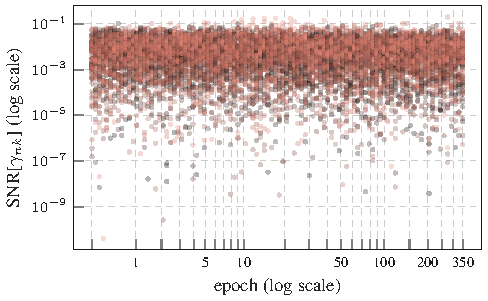
\includegraphics[width=\linewidth]{fig/exp13_plots/gammas_lambdas/cifar100_allcnnc_sgd_gammas.pdf}
\end{minipage}\hfill
\begin{minipage}{0.50\textwidth}
\centering
% WONTFIX: TeX memory exceeds!
% \plotGammasLambdas{cifar100}{allcnnc}{sgd}{lambdas}
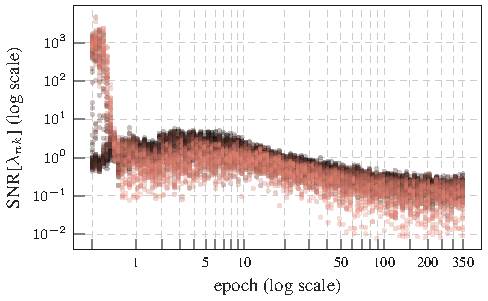
\includegraphics[width=\linewidth]{fig/exp13_plots/gammas_lambdas/cifar100_allcnnc_sgd_lambdas.pdf}
\end{minipage}

\vspace{3mm}

\textbf{\cifarhun \allcnnc \adam}\\[1mm]
\begin{minipage}{0.50\textwidth}
\centering
% WONTFIX: TeX memory exceeds!
% \plotGammasLambdas{cifar100}{allcnnc}{adam}{gammas}
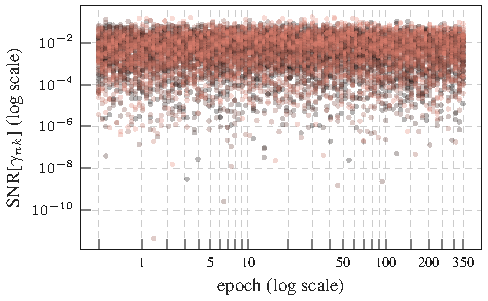
\includegraphics[width=\linewidth]{fig/exp13_plots/gammas_lambdas/cifar100_allcnnc_adam_gammas.pdf}
\end{minipage}\hfill
\begin{minipage}{0.50\textwidth}
\centering
% WONTFIX: TeX memory exceeds!
% \plotGammasLambdas{cifar100}{allcnnc}{adam}{lambdas}
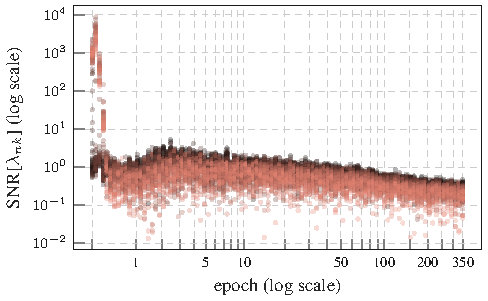
\includegraphics[width=\linewidth]{fig/exp13_plots/gammas_lambdas/cifar100_allcnnc_adam_lambdas.pdf}
\end{minipage}

\caption{\textbf{Directional SNRs (2):}
SNR along each of the mini-batch \ggn{}'s top-$C$ eigenvectors during training for all test problems.
At fixed epoch, the SNR for the most curved direction is shown in
{\protect\tikz{\protect\draw[white,fill={light_red},line width=0mm] (0,0) circle (.8ex);}}
and for the least curved direction in
{\protect\tikz{\protect\draw[white,fill={black}] (0,0) circle (.8ex);}}.
}
\label{fig:directional_derivatives_2}
\end{figure}

%%% Local Variables:
%%% mode: latex
%%% TeX-master: "../main"
%%% End:
